\section{Validation}
% Discuss different ways of validating the terrain.
% Describe what we want, and why we want this
    % See rivers from the fixed-point

\subsection{Object segmentation}
When validating the terrain, we want to make a distinction between different types of objects, such as the difference between the ground and rivers, or between the sky and placement objects. To solve this we use object segmentation, which is regularly used in computer vision \cite{kirillov_panoptic_2019}. In object segmentation we make a distinction between semantic segmentation, where all objects of the same type have the same colour, and panoptic segmentation, where each object has a different colour, regardless of it's type.

In our implementation we use a custom shader to colour the individual objects. When analysing the resulting image, we use pixel counting to find the relative size of the object in the view.

An example of applying image segmentation on a landscape is shown in figure \ref{fig:segmentation}. In this image we can see the original landscape on the top-left, and the segmented images on the right. The top image shows the object segmentation where the different kinds of placement object have a shared colour. The bottom image shows panoptic segmentation, where each object has an individual colour.

\begin{figure}
    \begin{subfigure}{.5\textwidth}
        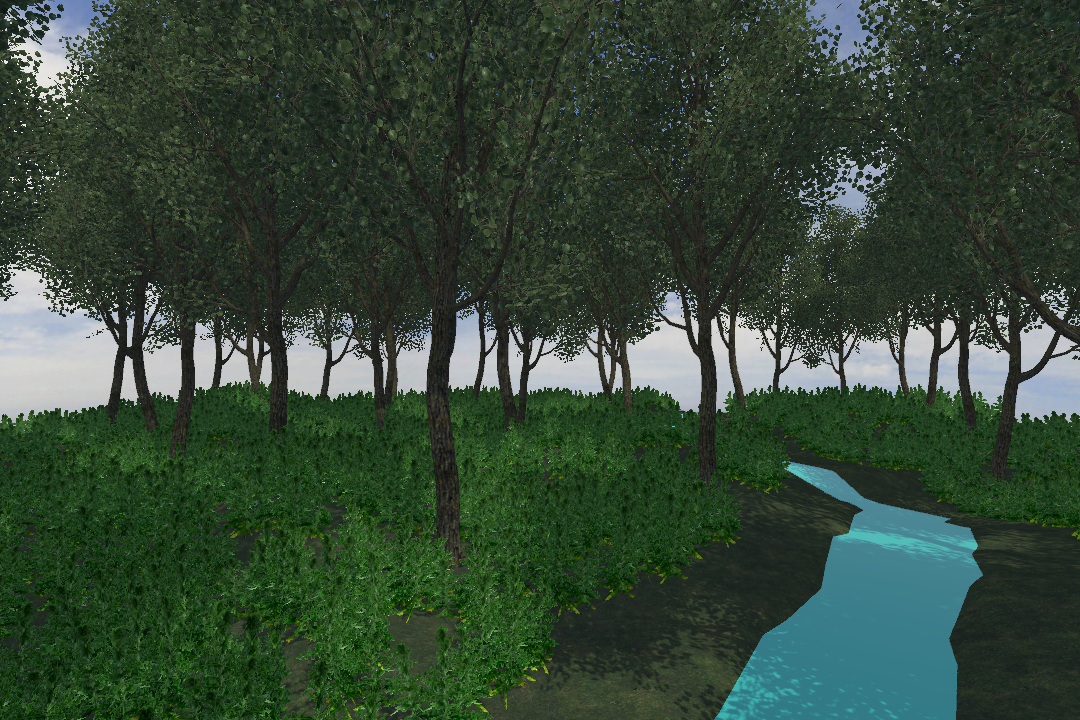
\includegraphics[width=\linewidth]{figures/validation/world_regular.png}
    \end{subfigure}
    \begin{subfigure}{.5\textwidth}
        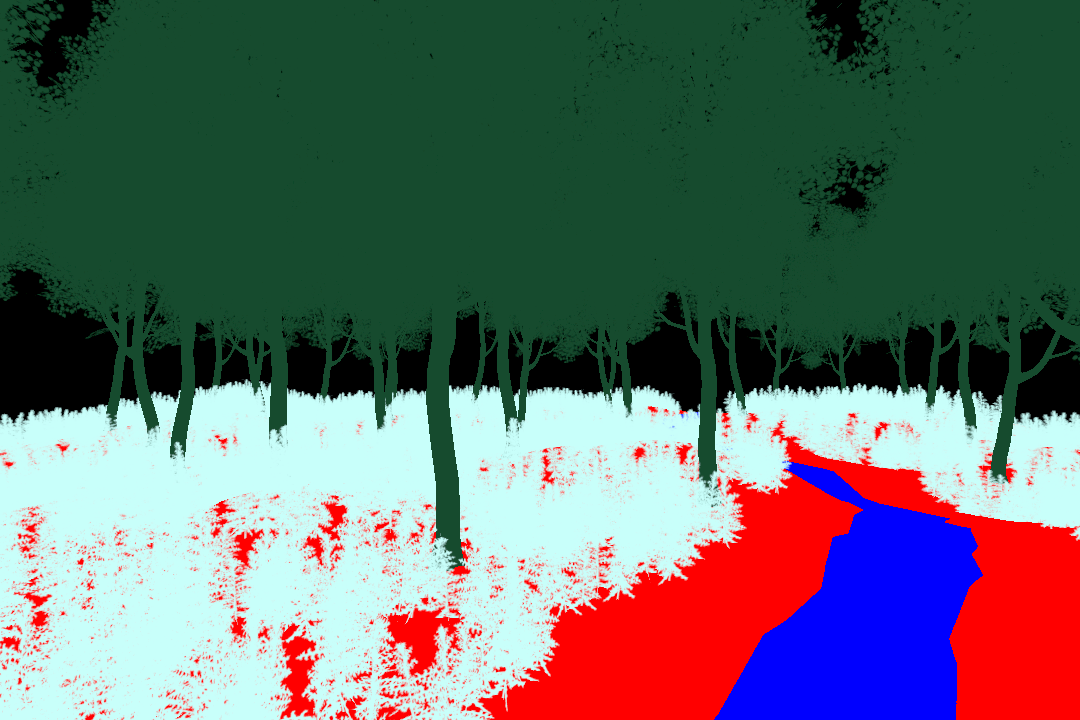
\includegraphics[width=\linewidth]{figures/validation/world_segmented.png}
    \end{subfigure}
    \hspace*{.5\linewidth}\begin{subfigure}{.5\textwidth}
        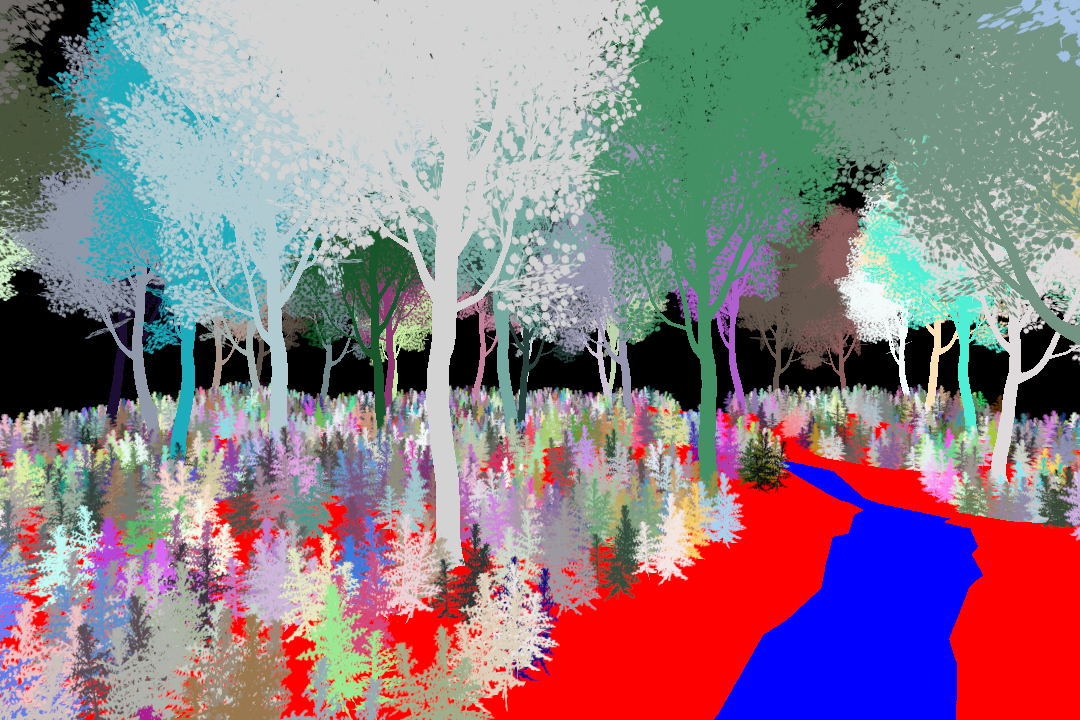
\includegraphics[width=\linewidth]{figures/validation/world_segmented_all.png}
    \end{subfigure}
    \caption{Example of object segmentation (up) and panoptic segmentation (down) on a generated terrain (left)}
    \label{fig:segmentation}
\end{figure}

% Introduce the task of object segmentation, and show how we use it to convert a regular image into a segmented image

\subsection{Presence and visibility of rivers} \todo{Show that this parameter can be used for estimation}
To show the visibility of the river in the landscape we analyse the proportion of the river in the terrain. As placement objects can obscure both a river and the terrain, this analysis is performed without the placement objects enabled.

To calculate the visibility of the river, the view of the camera is rendered with object segmentation, and from the pixels in the image the proportion of river against the entire terrain is calculated.

\subsubsection{Testing the visibility of rivers}
To test the visibility of the river, we take 500 samples of generated terrain, of which we calculate the percentage of terrain covered by the river. The result of this experiment is show in figure \ref{fig:river-visibility}. In these results, we see that the visibility of the river is very low, with more than 60\% of the samples being less than 5\%. One of the experiments where there is no river visible is shown in figure \ref{fig:river-visibility-results-low}. The generated terrain is shown in figure \ref{fig:river-visibility-results-low-world}. As seen, the generated river is very short, and only shown in the corner of the world. Because of this, it is not visible in the world. The world with the most visible river is shown in figure \ref{fig:river-visibility-results-high}. This river runs close to the camera, and therefore has a high visibility.

\begin{figure}
    \centering
    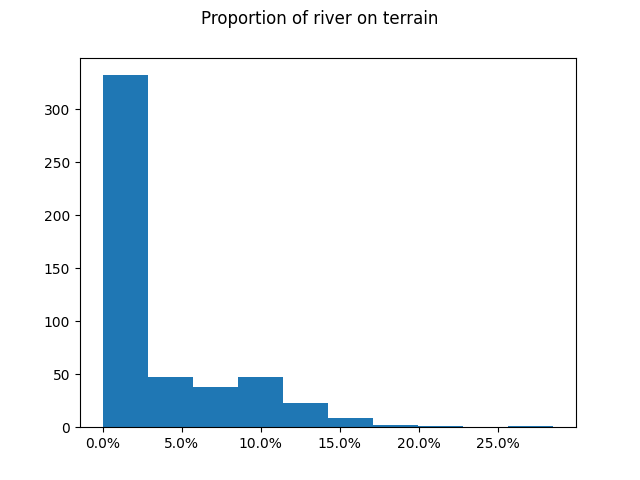
\includegraphics[width=0.8\linewidth]{figures/validation/2024-11-18_01-58-45_histogram.png}
    \caption{Histogram of the results of the river visibility test}
    \label{fig:river-visibility}
\end{figure}

\begin{figure}
    \begin{subfigure}{.5\textwidth}
        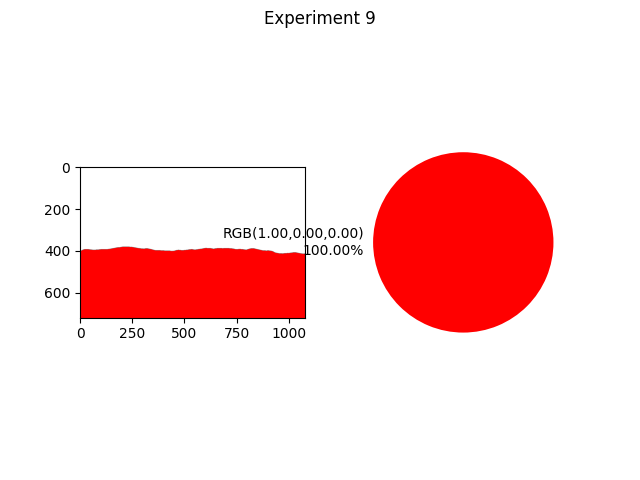
\includegraphics[width=\linewidth]{figures/validation/2024-11-18_01-58-45_9.png}
        \caption{Segmented view of a terrain without visible river}
        \label{fig:river-visibility-results-low}
    \end{subfigure}
    \begin{subfigure}{.5\textwidth}
        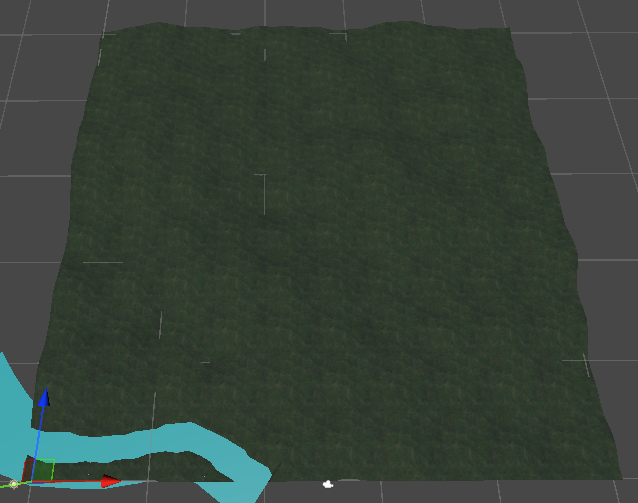
\includegraphics[width=\linewidth]{figures/validation/Bad river.png}
        \caption{Terrain of the view without a visible river}
        \label{fig:river-visibility-results-low-world}
    \end{subfigure}
    \begin{subfigure}{.5\textwidth}
        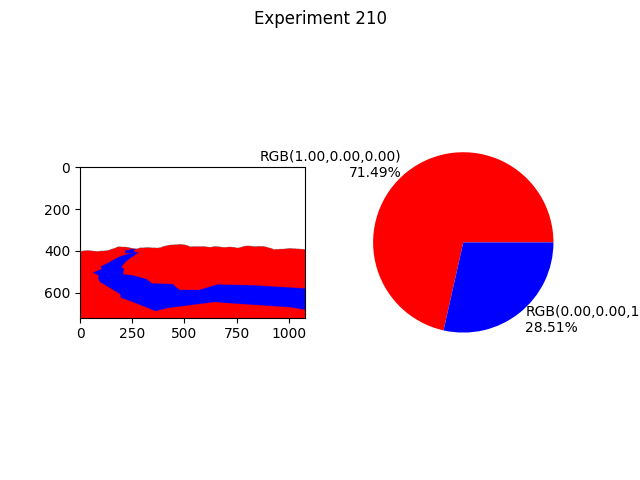
\includegraphics[width=\linewidth]{figures/validation/2024-11-18_01-58-45_210.png}
        \caption{Segmented view of terrain with the most visible river}
        \label{fig:river-visibility-results-high}
    \end{subfigure}
    \begin{subfigure}{.5\textwidth}
        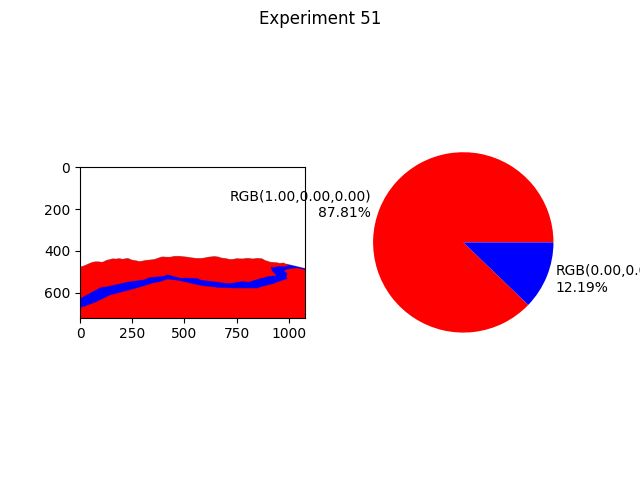
\includegraphics[width=\linewidth]{figures/validation/2024-11-18_01-58-45_51.png}
        \caption{Segmented view of terrain with medium visible river}
        \label{fig:river-visibility-results-medium}
    \end{subfigure}
    \label{fig:river-visibility-results}
\end{figure}

\subsubsection{Improving the visibility of rivers}
In the previous tests we kept the camera at a fixed position, namely on the centre of one side of the terrain. Instead of generating the terrain multiple times, the camera can be placed on any of the four sides of the terrain. This results in a different perspective on the terrain and therefore a different view on the river.

To test the improvement of this system, we perform the river visibility experiment, but for each terrain we calculate the visibility for each camera position, and take the camera position with the largest visibility. The histogram with the results of the experiments can be seen in figure \ref{fig:river-visibility-optimized}. From the results it shows that checking different camera positions does result in a terrain having a more visible river. Instead of more than 60\% of the experiments having no visible or nearly invisible river, selecting a different camera position has only 40\% of samples with a nearly invisible river. Although this method results in some terrains with a very large portion of water, with the largest proportion being 40\%, the largest increase in samples occurs between 10\% and 20\%.

\begin{figure}
    \centering
    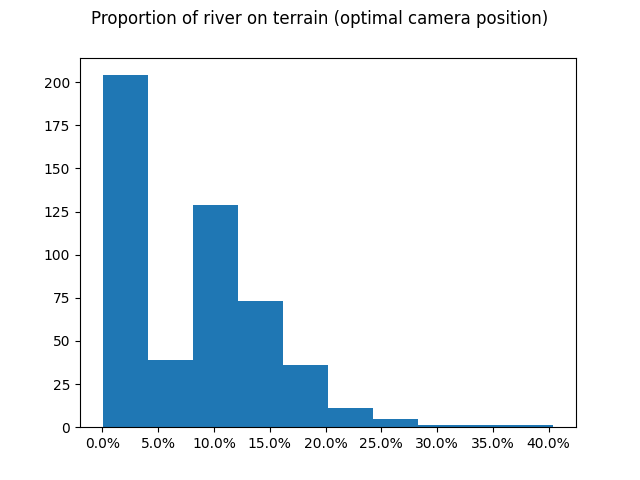
\includegraphics[width=0.8\linewidth]{figures/validation/2024-11-18_02-34-03_histogram.png}
    \caption{Histogram of the results of the river visibility test with the best camera position.}
    \label{fig:river-visibility-optimized}
\end{figure}


% Describe why we want to be able to see the rivers.
% Segmentation on terrain/water (not using placements)
% Show how we can find the proportion of surface that is river.
% Show examples of good/bad river representation.

\subsection{Single-object occlusion}

